\chapter{Data Foundation}
\label{data}
In this chapter the provided datasets from the previously mentioned street information systems and the FCD provider will be elaborated. In the beginning an overview of FCD in general and the available dataset is given. To give an overview about which results can be expected, the incident datasets from BAYSIS and ArbIS are presented with descriptive statistic. The most relevant parameters of the datasets will be elaborated and illustrated. The parameters are also categorized in the variable types defined in \cref{correlation_variable_types}.

\section{Floating-Car-Data (FCD)}
\label{dataset_fcd}
As described in \cref{introduction_continuous_floating_data}, \acrshort{fcd} represents the movement of vehicles and can be used to calculate vehicle speeds and trajectories. The provided dataset contains the aggregated absolute and relative speeds for highways and state streets, calculated from \acrshort{fcd} data. The process of speeds estimation with \acrshort{fcd} data is explained in detail by Felix Rampe in chapter 4 of his thesis \textit{Traffic Speed Estimation and Prediction Using Floating Car Data} \parencite{Rempe2018}, but goes beyond the scope of this thesis. The FCD is then mapped onto the HERE \parencite{HERE2020} network, to be compliant with the geolocation system used in the project. Each of these aggregated speeds now represents the mean speed over a three-minute time interval on the corresponding road section. This arrangement of speeds for each time step and space step can be called speed matrix and is the base data for the congestion detection. Figure \ref{img:speedMatrixPlot_mutipleMixedClusters} shows a visual representation a speed matrixes with the horizontal axes being the spatial extend and the vertical axes the time extend.
% TODO add more info about FCD if there is time 
% https://athene-forschung.unibw.de/doc/127445/127445.pdf
% Traffic Speed Estimation and Prediction Using Floating Car Data.pdf

\begin{figure}[ht]
	\centering
	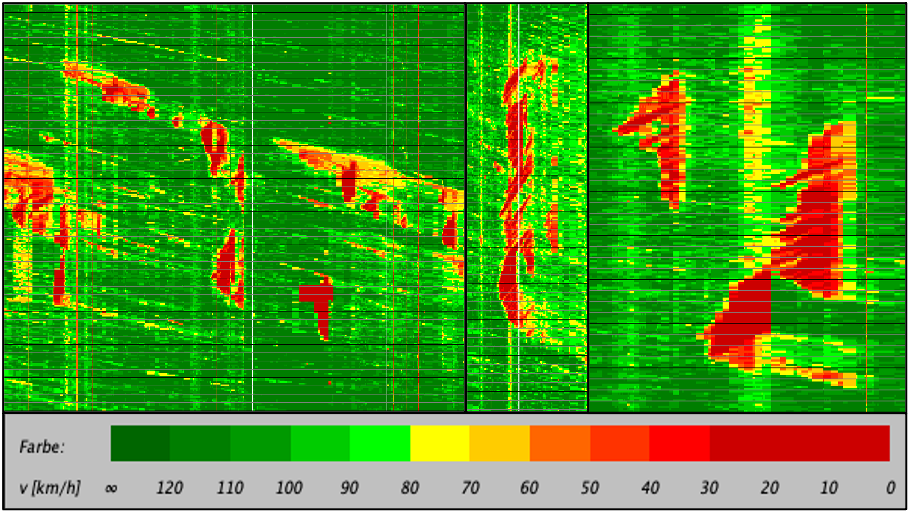
\includegraphics[scale=0.7]{images/SpeedMatrixPlot_mutiple}
	\caption{Speed matrix plots of processed FCD data, showing different jam clusters}
	\label{img:speedMatrixPlot_mutipleMixedClusters}
\end{figure}

Deep greens represent free flowing traffic with 130 km/h, according to the norm speed on highways set the legislator in Germany (in german called “Richtgeschwindigkeit”). The speed scale then develops linearly downwards to deep red indicating traffic with 30 km/h or less. The observer will clearly recognize the jams represented by the clusters of red and orange cells in the \cref{img:speedMatrixPlot_mutipleMixedClusters}. The vehicle trajectory through space and time can be recognize on the angled extends from the top left to the bottom right. From this visual clarity speed matrix and the precision on 3-minute intervals it can be concluded that a comprehensive algorithmic approach should be able to detect such congestion events. This being said, the dataset does contain defects in the form of missing values for complete road sections, which can interfere with detection algorithm. Another defect type would be an obviously wrong speed block, meaning sudden speed drops or jumps to areas of identical speeds with an abnormal temporal and spatial extend, which then have to be ignored during processing. 

\section{Accident Data (BAYSIS)}
\label{dataset_baysis}
The \acrfull{baysis} as described in \cref{introduction_street_information_systems}, collects a wide range of different information types, one of them being accidents with the corresponding police reports. The provided export from BAYSIS contains all accidents of the year 2019 on the Bavarian highway network, which are 10262 records in number. Each accident report includes a variety of specifications which covers environmental indicators like weather or light situation, accident characteristics like accident type, collision object or cause, as well as information over the involved persons like nationality, age and gender. In total, one report contains 132 values describing the accident, participant and environment. As there shouldn't be formed a stereotype of accident participant but rather significant accident characteristics or environmental factors be found, most of the descriptive values for the involved persons are not considered. Variables which contain no values or a single values and fall under the uncertainty threshold (see \cref{correlation_uncertainty}) are also neglected. From this curtailed pool of correlate able and analyze able characteristics all parameters that have a logical significance with causes or effects of an accident will be considered in the analysis. The referred figures are available as larger prints in the appendix \cref{appendix_baysis} for better readability, as they do not properly fit in the text. 

\begin{figure}[ht]
	\centering
	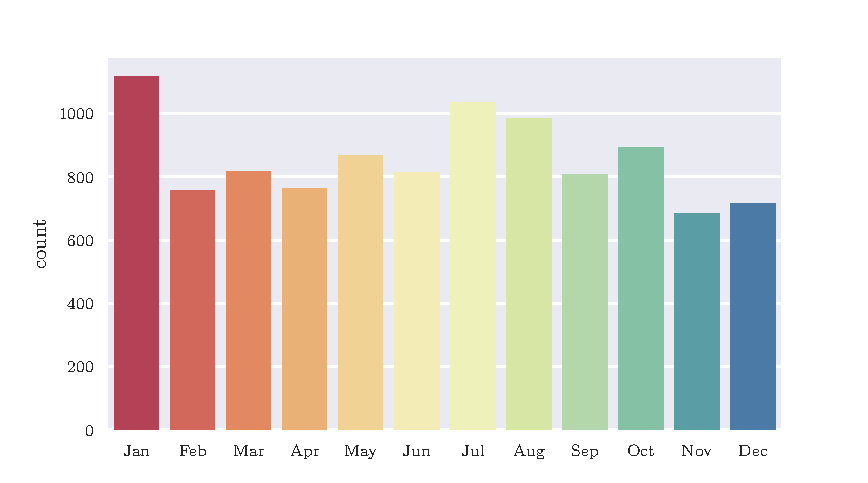
\includegraphics[scale=0.9]{CorrAnalysis/data/BAYSIS/01_dataset/plots/baysis_dataset_hist_month}
	\caption{Distribution of accident counts by months}
	\label{img:baysis_dataset_dist_month}
\end{figure}
A look on the monthly distribution of accidents recorded by BAYSIS (see \cref{img:baysis_dataset_dist_month}) shows that that the months of January, July and August show a considerably high number of accidents, with respectively 31\,\%, 21\,\% and 15\,\% increase over the mean count of 855 accidents per month. The increased number in January can be explained with the increased number of accidents due to ice and snow conditions, which reduces traction on roads and can lead to uncontrollable vehicle behavior. Also the reduced visibility during snow falls increases accident numbers. In July and August the increased traffic volume because of public holidays is the most probable explanation for the higher number of accidents. Another valuable distribution is the number of accidents per road (see \cref{img:baysis_dataset_dist_highway}). The roads A3, A9 and A8 show a relative high count of accidents whereas the road A71 and beneath only have a small number accidents.
\begin{figure}[ht]
	\centering
	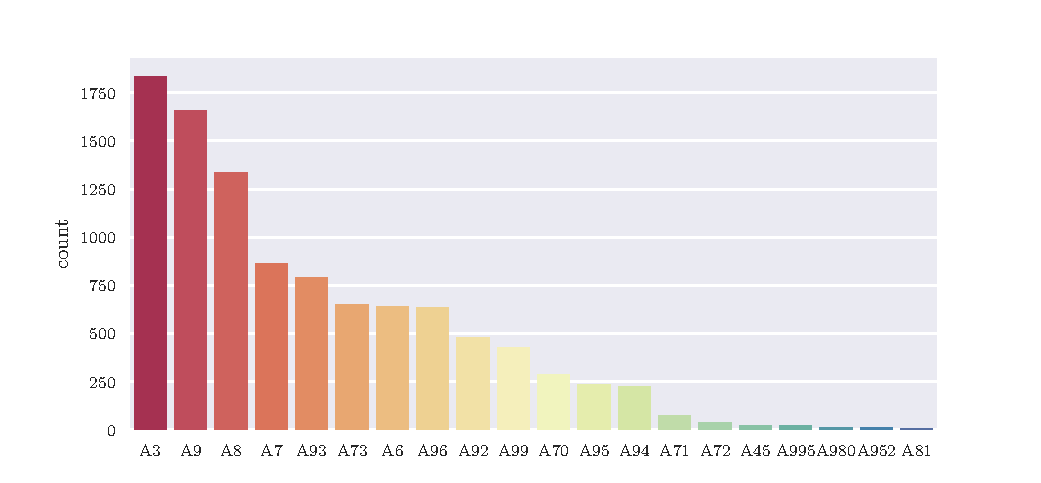
\includegraphics[scale=0.75]{CorrAnalysis/data/BAYSIS/01_dataset/plots/baysis_dataset_hist_highway}
	\caption{Distribution of accident counts by highway}
	\label{img:baysis_dataset_dist_highway}
	\vspace{-8mm}
\end{figure}
\paragraph{Kat}
\label{baysis_dataset_Kat}
The accident category (shown in \cref{tbl:baysis_dataset_Kat} and visualized in \cref{img:baysis_dataset_Kat}), describes which damages or injuries can be associated with the accident. It ranges from accidents with just damaged property to lightly and heavily injured and even deathly accidents. The distribution develops from lowest to highest counts, in order of gravity of the category. The variable consists of four values, which can be ordered and is therefore ordinal.
\begin{table}[ht!]
	\centering
	\small
	\begin{tabular}{c|c|c|l} 
		\toprule
		Code & \textbf{Kat} & [\%] & Description \\ 
		\midrule
 		0 	& - 	& 	-	& Minor Accident  \\
 		1 	& 76 	& 0.7 	& Accident with deaths  \\ 
 		2 	& 600	& 5.8	& Accident with heavily injured  \\
 		3 	& 2685	& 26.2	& Accident with lightly injured  \\
		7 	& 6900	& 67.2	& Accident with property damage  \\
		\bottomrule
	\end{tabular}
	\caption{Descriptive of \textbf{Kat}}
	\label{tbl:baysis_dataset_Kat}
	% \vspace{-8mm}
\end{table}
\paragraph{Typ}
\label{baysis_dataset_Typ}
The accident type variable (shown in \cref{tbl:baysis_dataset_Typ} and visualized in \cref{img:baysis_dataset_Typ}) incorporates different kinds of traffic movements from straight driving to turning movements or merging. It describes during which kind of movement the accident happened. Beside of an 80\,\% share of accidents related to driving or straight driving situations, the parameter does not indicate any other features. The variable does not show any order and is therefore of a nominal type.
\begin{table}[!ht]
	\centering
	\small
	\begin{tabular}{c|c|c|l} 
		\toprule
		Code & \textbf{Typ} & [\%] & Description \\ 
		\midrule
 		1 & 2820	& 27.5	& Driving accident \\ 
 		%2 & 1		& < 0.1 & Turning accident \\
 		3 & 373		& 3.6 	& Merging / Crossing accident \\
 		4 & 10		& 0.1	& Crossing over accident \\
 		5 & 160 	& 1.6	& Accident in standing traffic \\
 		6 & 5285	& 51.5	& Accident in straight traffic \\
		7 & 1612	& 15.7 	& Other \\
		\bottomrule
	\end{tabular}
	\caption{Descriptive of \textbf{Typ}}
	\label{tbl:baysis_dataset_Typ}
	\vspace{-8mm}
\end{table}
\paragraph{Betei}
\label{baysis_dataset_Betei}
The distribution of the number of involved persons (shown in \cref{tbl:baysis_dataset_Betei} and visualized in \cref{img:baysis_dataset_Betei}) shows that more than 97\,\% of all accidents have three or less involved persons, which is supported by a mean of 1.9 involved persons per accident in general. The major share of two involved persons makes up for 59\,\% and the second biggest of one involved person for 30\,\% of the total count. Because of the increasing order of values, the variable is of an ordinal type.
\begin{table}[!ht]
	\centering
	\small
	\begin{tabular}{r|ccccccc} 
		\toprule
		 			& 1		& 2		& 3		& 4		& 5		& 6  	& > 7\\ 
		\midrule
		\textbf{Betei}		& 2768	& 6047	& 1085	& 235	& 72 	& 24	& 30 \\ 
 		Freq. 	& 27.0	& 58.9	& 10.6 	& 2.3	& 0.7 	& 0.2 	& 0.1 \\
		\bottomrule
	\end{tabular}
	\caption{Descriptive of \textbf{Betei}}
	\label{tbl:baysis_dataset_Betei}
	\vspace{-8mm}
\end{table}
\paragraph{UArt}
\label{baysis_dataset_UArt}
The accident cause type is defined by the two variables \textbf{UArt1} and \textbf{UArt2} (shown in \cref{tbl:baysis_dataset_UArt} and visualized in \cref{img:baysis_dataset_UArt}), whereat the first is the more suitable one. They describe the type of collision cause and presents two major sets. One being the accidents with waiting, stopping and starting vehicles in the same lane, which describe typical collision accidents during congested traffic. The other being the accidents in the next left or right lane, which describe common lane changing collisions. Accidents with cross traffic, pedestrians or opposite traffic are relatively uncommon. The variable does not show any order and is therefore of a nominal type.
\begin{table}[ht]
	\centering
	\small
	\begin{tabular}{c|c|c|c|l} 
		\toprule
		Code & \textbf{UArt1} & \textbf{UArt2} & Freq. & Description \\ 
		\midrule
 		1 & 466		& 13	& 4.2  & Collision with starting, standing or stopping vehicle  \\ 
 		2 & 2111	& 44 	& 18.8 & Collision with ahead and waiting vehicle  \\
 		3 & 2873	& 140	& 26.3 & Collision with vehicle on separate lane in same direction  \\
 		4 &	16		& 4		& 0.2   & Collision with vehicle going in opposite direction  \\
 		5 & 240		& 12	& 2.2  & Collision with turning or crossing vehicle  \\
 		6 & 19		& 1		& 0.2   & Collision between vehicle and pedestrian  \\
 		7 & 411		& 42	& 4.0  & Collision with obstacle  \\
 		8 & 1728	& 381	& 18.4 & Deviation to the right  \\
 		9 & 1446	& 517	& 17.1 & Deviation to the left  \\
		0 & 951		& 42	& 8.7  & Other  \\
		\bottomrule
	\end{tabular}
	\caption{Descriptive of \textbf{UArt}}
	\label{tbl:baysis_dataset_UArt}
	%\vspace{-8mm}
\end{table}
\paragraph{AUrs}
\label{baysis_dataset_AUrs}
The summarized distribution of the parameters \textbf{AUrs1} and \textbf{AUrs2} (shown in \cref{tbl:baysis_dataset_AUrs} and visualized in \cref{img:baysis_dataset_AUrs}) shows that the variable is not much distributed and only a small number of categories hold a relevant sample size. Any correlation to this parameter needs to interpreted with caution, due to the high uncertainty. The variable is of a nominal type.
\begin{table}[ht]
	\centering
	\small
	\begin{tabular}{c|c|c|c|l}
		\toprule
		Code & \textbf{AUrs1} & \textbf{AUrs2} & [\%] & Description \\ 
		\midrule
		%70 & - 	& -		&     & Slippery street due to oil \\
		%71 & -		& -		&     & Slippery street due to dirt \\
		72 & 618	& -		& 33  & Slippery street due to snow or ice \\
		73 & 855	& 45	& 48  & Slippery street due to rain \\
		%74 & -		& -		&     & Slippery street due to other objects \\
		75 & 11		& 12	& 1.2 & Cart track due to rain, snow or ice \\
		76 & 10		& 3		& 0.7 & Other condition of road \\
		%77 & 1		& -		&     & Un-regular condition of traffic signs \\
		%78 & -		& -		&     & Bad lighting of street \\
		%79 & -		& -		&     & Bad safety on train crossing \\
		%80 & 1		& 3		&     & Visibility issues due to fog \\
		81 & 4		& 17 	& 1.1 & Visibility issues due to rain or hail \\
		82 & 24		& -		& 1.3 & Visibility issues due to sun or glare \\
		%83 & 2		& 3		&     & Crosswind \\
		84 & 1		& 14	& 0.8 & Visibility issues due to storm \\
		%85 & -		& -		&     & Unsafe roadwork \\
		86 & 21		& -		& 1.1 & Wild animals \\
		%87 & 1		& -		&     & Other animals \\
		88 & 134	& 4		& 7.4 & Other obstacles \\
		89 & 97		& 4		& 5.4 & Other causes \\
		% Count[1] 0 = 8435 / Count[2] 0 = 10156
		\bottomrule
	\end{tabular}
	\caption{Descriptive of \textbf{AUrs}}
	\label{tbl:baysis_dataset_AUrs}
	\vspace{-8mm}
\end{table}
\paragraph{AufHi}
\label{baysis_dataset_AufHi}
The obstacle collision distribution (shown in \cref{tbl:baysis_dataset_AufHi} and visualized in \cref{img:baysis_dataset_AufHi}) reveals that in most collision accidents cars hit the guardrails. The other categories are rather uncommon. With 1,4\,\% of accidents without any collision, it can be stated that in most cases a collision is part of an accident. The counts of the remaining categories are insignificant. The variable does not show any order and is therefore of a nominal type.
\begin{table}[ht]
	\centering
	\small
	\begin{tabular}{c|c|c|l} 
		\toprule
		Code & \textbf{AufHi} & [\%] & Description \\ 
		\midrule 
		0 & 16 		& 0.2	& Single tree \\
		1 & 12 		& 0.1	& Pillar \\
		%2 & 5 		& < 0.1	& Abutment \\
		3 & 3041	& 29.6	& Guardrail \\
		4 & 534		& 5.2	& Other object \\
		5 & 144		& 1.4	& No collision \\
		%7 & 2		& < 0.1	& Tree line or alley \\
		8 & 26		& 0.3	& Tree group or forest \\
		9 & 52		& 0.5	& Busches \\
		\bottomrule
	\end{tabular}
	\caption{Descriptive of \textbf{AufHi}}
	\label{tbl:baysis_dataset_AufHi}
	\vspace{-8mm}
\end{table}
\paragraph{Alkoh}
\label{baysis_dataset_Alkoh}
The alcohol involvement indication variable only contains one variables of ($1 = yes$), whereas an empty variable referred to $no$ or $unknown$. It reveals that only 2.2\,\% of accidents have one or more involved persons with measurable blood alcohol. The variable only has two unique values and is therefore dichotomous.
\paragraph{Char}
\label{baysis_dataset_Char}
The variable Char1 and Char2 (shown in \autoref{tbl:baysis_dataset_Char} and visualized in \ref{img:baysis_dataset_Char}) describes the characteristics of the street where the accident happened. Since only highway are considered, the type of \textit{Crossing}, \textit{Property} and \textit{Roundabout} is expected to be zero. The variable is not ordered and therefore of a nominal type.  
\begin{table}[ht]
	\centering
	\small
	\begin{tabular}{c|c|c|c|l}
		\toprule
		Code & \textbf{Char1} & \textbf{Char1} & [\%] & Description \\ 
		\midrule
		%1 & - 	& -		& 		& Crossing \\
	    2 & 42	& -		& 2.9	& Entry / Exit \\
	    %3 & 1	& -		&		& Property access \\
	    4 & 380	& -		& 26	& Incline \\
	    5 & 371	& -		& 25.4	& Decline \\
	    6 & 404	& 263	& 45.7	& Curve \\
		%7 & -	& -		&		& Roundabout \\
		\bottomrule
	\end{tabular}
	\caption{Descriptive of \textbf{Char}}
	\label{tbl:baysis_dataset_Char}
	\vspace{-8mm}
\end{table}
\paragraph{Bes}
\label{baysis_dataset_Bes}
The variables \textbf{Bes1}, \textbf{Bes2} and \textbf{Bes3} further define the street characteristic mentioned above, although they only contain one variable, referring to the category \textit{Roadwork}. As the variable is not distributed it is not suitable for correlation analysis, but can be used to validate the roadwork matching performance.
% \begin{table}[ht]
% 	\centering
% 	\begin{tabular}{c|l}  
% 		1 & Confusing \\ 
% 		2 & Level crossing \\
% 		3 & Pedestrian crossing \\
% 		4 & Pedestrian passage \\
% 		5 & Bus-stop \\
% 		6 & Roadwork \\
% 		7 & Calm traffic area \\
% 		8 & RAV on street \\
% 		9 & RAV separate \\
% 		0 & RAV obligatory \\
% 	\end{tabular}
% 	\caption{Identifier and description of 'Bes'}
% 	\label{table:baysis_dataset_Bes}
% \end{table}
\paragraph{Lich}
\label{baysis_dataset_Lich}
The light situation variable (shown in \cref{tbl:baysis_dataset_Lich} and visualized in \cref{img:baysis_dataset_Lich}) describes the lighting condition at the time of the accident. The variable \textbf{Lich1} describes the nature light setting, when \textbf{Lich2} describes if the street light was working. Because \textbf{Lich1} can be ranked from best to worst lighting is of an ordinal type. \textbf{Lich2} only has two values and is therefore dichotomous.
\begin{table}[ht]
	\centering
	\small
	\begin{tabular}{c|c|c|c|l}
		\toprule
		Code & \textbf{Lich1} & \textbf{Lich2} & [\%] & Description \\ 
		\midrule 
		0 & 6833 	& - 	& 51.7 & Daylight \\
		1 & 627 	& -		& 4.7  & Noon \\
		2 & 2560	& - 	& 19.4 & Darkness \\
		3 & - 		& 3005	& 22.8 & Street lighting working \\
		4 & - 		& 182	& 1.4  & Street lighting not working \\
		\bottomrule
	\end{tabular}
	\caption{Descriptive of \textbf{Lich}}
	\label{tbl:baysis_dataset_Lich}
	\vspace{-8mm}
\end{table} 
\paragraph{Zust}
\label{baysis_dataset_Zust}
The road condition parameter (shown in \cref{tbl:baysis_dataset_Zust} and visualized in \cref{img:baysis_dataset_Zust}) describes in which condition e.g. wet, dry, iced or slippery the road was at time of the accident. The condition can be ranked from best to worst and is therefore of an ordinal type.
\begin{table}[ht]
	\centering
	\small
	\begin{tabular}{c|c|c|c|l}
		\toprule
		Code & \textbf{Zust} & Count[2] & [\%] & Description \\ 
		\midrule 
		0 & 6851 	& -		& 66.9 & Dry \\ 
 		1 & 2606	& -		& 25.4 & Wet \\ 
 		2 & 582		& 207	& 7.7  & Ice \\
 		%3 & - 		& -		& & Slippery (oil, dirt, ...)  \\
	\end{tabular}
	\caption{Descriptive of \textbf{Zust}}
	\label{tbl:baysis_dataset_Zust}
	\vspace{-8mm}
\end{table}
\paragraph{Fstf}
\label{baysis_dataset_Fstf}
The variable references the lane on which the accident happened (shown in \cref{tbl:baysis_dataset_Fstf} and visualized in \cref{img:baysis_dataset_Fstf}). It names the number of lane from the right, the hard-shoulder or the wrong usage of a one-way street. It shows a ranked order of the lane number, but not with the two other types of hard-shoulder (\textit{S}) and one-way street (\textit{F}). It is therefore considered as nominal type.
\begin{table}[ht]
	\centering
	\small
	\begin{tabular}{c|c|c|l}
		\toprule
		Code & \textbf{Fstf} & [\%] & Description \\ 
		\midrule  
		1 & 2821 	& 27.5 	& first lane from the right \\
		2 & 4274 	& 41.7 	& second lane from the right \\
		3 & 1582 	& 15.4 	& third lane from the right \\
		4 & 150 	& 1.5 	& fourth lane from the right \\
		5 & 26 		& 0.3 	& firth lane from the right \\ 
 		S & 247 	& 2.4 	& on the hard-shoulder lane \\ 
		%F & 7 		& 0.1 	& on opened hard-shoulder lane \\
		\bottomrule
	\end{tabular}
	\caption{Descriptive of \textbf{Fstf}}
	\label{tbl:baysis_dataset_Fstf}
	\vspace{-8mm}
\end{table} 
\paragraph{WoTag}
\label{baysis_dataset_WoTag}
The variable of WoTag relates to the day of the week the accident happened (shown in \cref{img:baysis_dataset_WoTag}). It is debatable if week days can be ordered but for this analysis the parameter will be considered a nominal type.
\paragraph{FeiTag}
\label{baysis_dataset_FeiTag}
Only 157 accidents took place on a public holiday. This is not a feature itself but there could be a possible correlation to it, as the jams could be longer because of the increased traffic demand on holiday.

% \cref{tbl:baysis_variables} show all categorized parameters, relevant for the correlation analysis, with variable group, type and the format of the containing data. 
% \begin{table}[ht]
% 	\centering
% 	\small
% 	\begin{tabular}{c|c|c|c}
% 		\toprule
% 		\textbf{Variable} 	& \textbf{Group} 	& \textbf{Type} & \textbf{Format} \\
% 		\midrule
% 		Kat  		& categorical 	& ordinal 	& numeric\\
% 		\midrule
% 		Typ 		& categorical 	& nominal	& numeric\\
% 		\midrule
% 		Beteil 		& categorical 	& ordinal	& numeric\\
% 		\midrule
% 		UArt 		& categorical 	& nominal	& numeric\\
% 		\midrule
% 		AUrs 		& categorical 	& nominal	& numeric\\
% 		\midrule
% 		AufHi 		& categorical 	& nominal	& numeric\\
% 		\midrule
% 		Alkoh 		& categorical 	& dichotomous	& numeric\\
% 		\midrule
% 		Char 		& categorical 	& nominal	& numeric\\
% 		\midrule
% 		Bes 		& categorical 	& nominal	& numeric\\
% 		\midrule
% 		Lich 		& categorical 	& ordinal	& numeric\\
% 		\midrule
% 		Zust 		& categorical 	& ordinal	& numeric\\
% 		\midrule
% 		Fstf 		& categorical 	& nominal	& mixed\\
% 		\midrule
% 		WoTag 		& categorical 	& nominal	& text\\
% 		\midrule
% 		FeiTag 		& categorical 	& dichotomous	& numeric\\
% 		\bottomrule
% 	\end{tabular}
% 	\caption{Variable types of \acrshort{baysis} dataset}
% 	\label{tbl:baysis_variables}
% \end{table}

The designed evaluation tool utilizes a PostgreSQL database for its data storage. Therefore the BAYSIS data in form of \acrfull{csv} needs to be processed and converted into SQL data entities. Also, the data entities for each accident need to be uniform and comparable with the street network and other entities like roadworks, which makes it necessary to process and map the accidents onto our street network. After the necessary processing and import into the database, 7971 records end up being converted and persisted, which is equivalent to 77,6\,\% of the total number of accidents. This 22,4\,\% of data loss can be explained due to the conversion of from the BAYSIS geo-system to the HERE network, which tries to find a corresponding street network location to the legacy location of the BAYSIS dataset. If it is not able to locate the position of the BYSIS dataset on our street network, the record is discarded.

\section{Roadwork Data (ArbIS)}
\label{dataset_arbis}

The \acrfull{arbis} as described in \autoref{dataset_arbis} is a collection service of all roadworks or maintenance which is planned, ongoing or finished on the Bavarian street network. The dataset for 2019 contains close to 650.000 data-points which each describe the temporal and spatial extend, road name and number of closed lanes of a roadwork fragment. This fragmentation of events makes it hard to statically analyze this dataset since each roadwork is spitted into any number of fragments which are only linked by a roadwork identifier. Therefore the analysis of the dataset in this section is relatively basic. The import processing works similarly to the \acrshort{baysis} data in \autoref{dataset_baysis} and produces 282.839 roadwork events in the database after the aggregation of fragments. 

With 4500 long term and more than 40.000 short term building sites on German highways per year \parencite{LAPID2018,Stmi2020} road construction makes up for the majority of traffic obstructions during the summer months. Throughout the colder months, in which a majority of construction projects are not possible, snow clearings or long-term constructions are the main obstacles. This also means that the number and type of roadworks varies during the course of a year \parencite{Stmi2020}. 
\begin{figure}[ht]
	\centering
	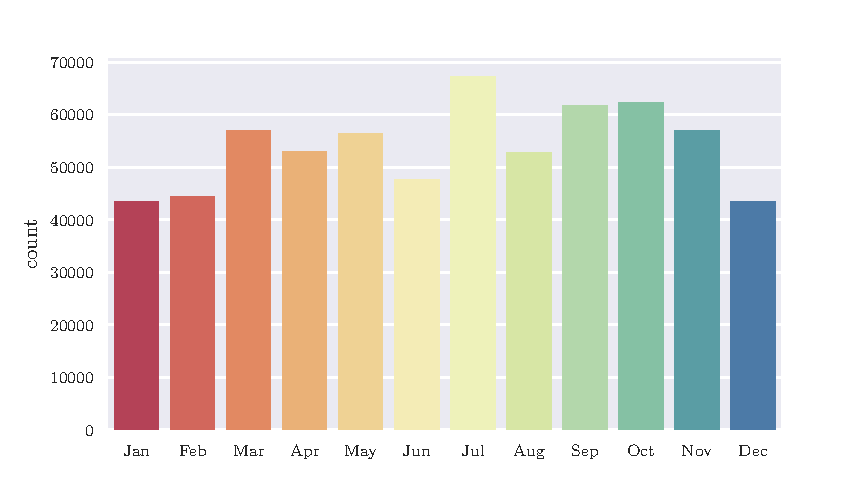
\includegraphics[width=0.7\textwidth]{../CorrAnalysis/data/ArbIS/01_dataset/plots/arbis_dataset_hist_month}
	\caption{Monthly distribution of roadwork fraction counts}
	\label{img:arbis_dataset_dist_month}
\end{figure}
The monthly distribution of roadworks in the year 2019 in figure \autoref{img:arbis_dataset_dist_month} supports this statement, since the winter months of January, February and December tend to have less roadwork that others. In July most of the roadwork is done. Similar to the BAYSIS data the road \textit{A3} and \text{A9} have the highest numbers of roadworks (shown in figure \autoref{img:arbis_dataset_dist_highway}).
\begin{figure}[ht]
	\centering
	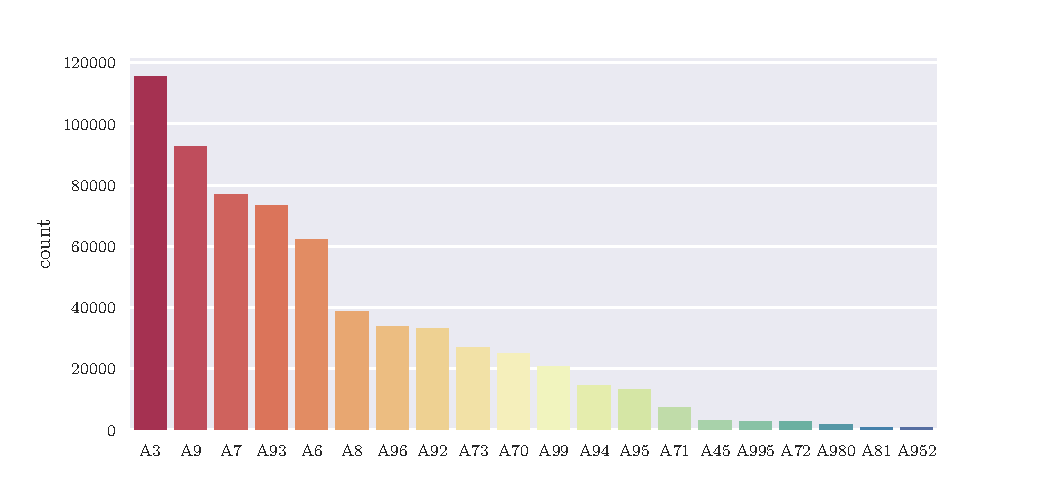
\includegraphics[width=0.7\textwidth]{../CorrAnalysis/data/ArbIS/01_dataset/plots/arbis_dataset_hist_highway}
	\caption{Distribution of roadwork fraction counts, by road}
	\label{img:arbis_dataset_dist_highway}
\end{figure}

\paragraph{AnzGesperrtFs} refers to the number of closed lanes for the time of the incident. The distribution shows that two states of zero and one block lane hold nearly 100\,\% of all samples. Since the variable can be ordered by the number of lanes, it is of an ordinal type.
\begin{table}[!ht]
	\centering
	\small
	\begin{tabular}{c|c|c} 
		\toprule
		\textbf{AnzGesperrtFs} & Count & [\%] \\ 
		\midrule
		% -1 & 3		& < 0.1 \\
		0  & 215977	& 33.4  \\ 
		1  & 430022	& 66.5  \\	 
		2  & 140	& < 0.1 \\ 
		3  & 81	 	& < 0.1 \\
		\bottomrule
	\end{tabular}
	\caption{Descriptive of \textbf{AnzGesperrtFs}}
	\label{tbl:arbis_dataset_AnzGesperrtFs}
	\vspace{-8mm}
\end{table}

\paragraph{Einzug} describes the shift of the road way due to physical changes measured in the number of lanes. It ranges from one to five lanes, where one, two and five are equally frequent. The variable is limited, can be sorted and therefore is of an ordinal type.
\begin{table}[!ht]
	\centering
	\small
	\begin{tabular}{c|c|c} 
		\toprule
		\textbf{Einzug} & Count & [\%] \\ 
		\midrule
		1 & 230192 & 35.6  \\
		2 & 201289 & 31.1  \\ 
		3 & 728	   & 0.1   \\ 
		4 & 1	   & < 0.1 \\ 
		5 & 214543 & 33.2  \\
		\bottomrule
	\end{tabular}
	\caption{Descriptive of \textbf{Einzug}}
	\label{tbl:arbis_dataset_Einzug}
\end{table}

Since \textbf{Length} and \textbf{Duration} are not part of the original dataset, they are calculated from the dataset parameters \textit{VonKilometer} / \textit{BisKilometer} and \textit{Von} / \textit{Bis} respectively. They are measurements and therefore are of an interval type.

% \cref{table:arbis_variables} shows all categorized parameters, relevant for the correlation analysis, with variable group, type and the format of the containing data.	
% \begin{table}[!ht]
% 	\centering
% 	\begin{tabular}{c|c|c|c}
% 		\toprule
% 		\textbf{Variable} 	& \textbf{Group} 	& \textbf{Type} 		& \textbf{Format} \\
% 		\midrule
% 		AnzGesperrtFs  	& categorical 	& ordinal 	& numeric\\
% 		\midrule
% 		Einzug  		& categorical 	& ordinal 	& numeric\\
% 		\midrule
% 		Length  		& continuous 	& interval 	& numeric\\
% 		\midrule
% 		Duration  		& continuous 	& interval 	& numeric\\
% 		\bottomrule
% 	\end{tabular}
% 	\caption{Variable types of \acrshort{baysis} dataset}
% 	\label{table:arbis_variables}
% \end{table}
